\documentclass{standalone}
\usepackage{tikz}
\usetikzlibrary{patterns, positioning}
\usepackage[sfdefault]{ClearSans} %% option 'sfdefault' activates Clear Sans as the default text font
\usepackage[T1]{fontenc}

\begin{document}
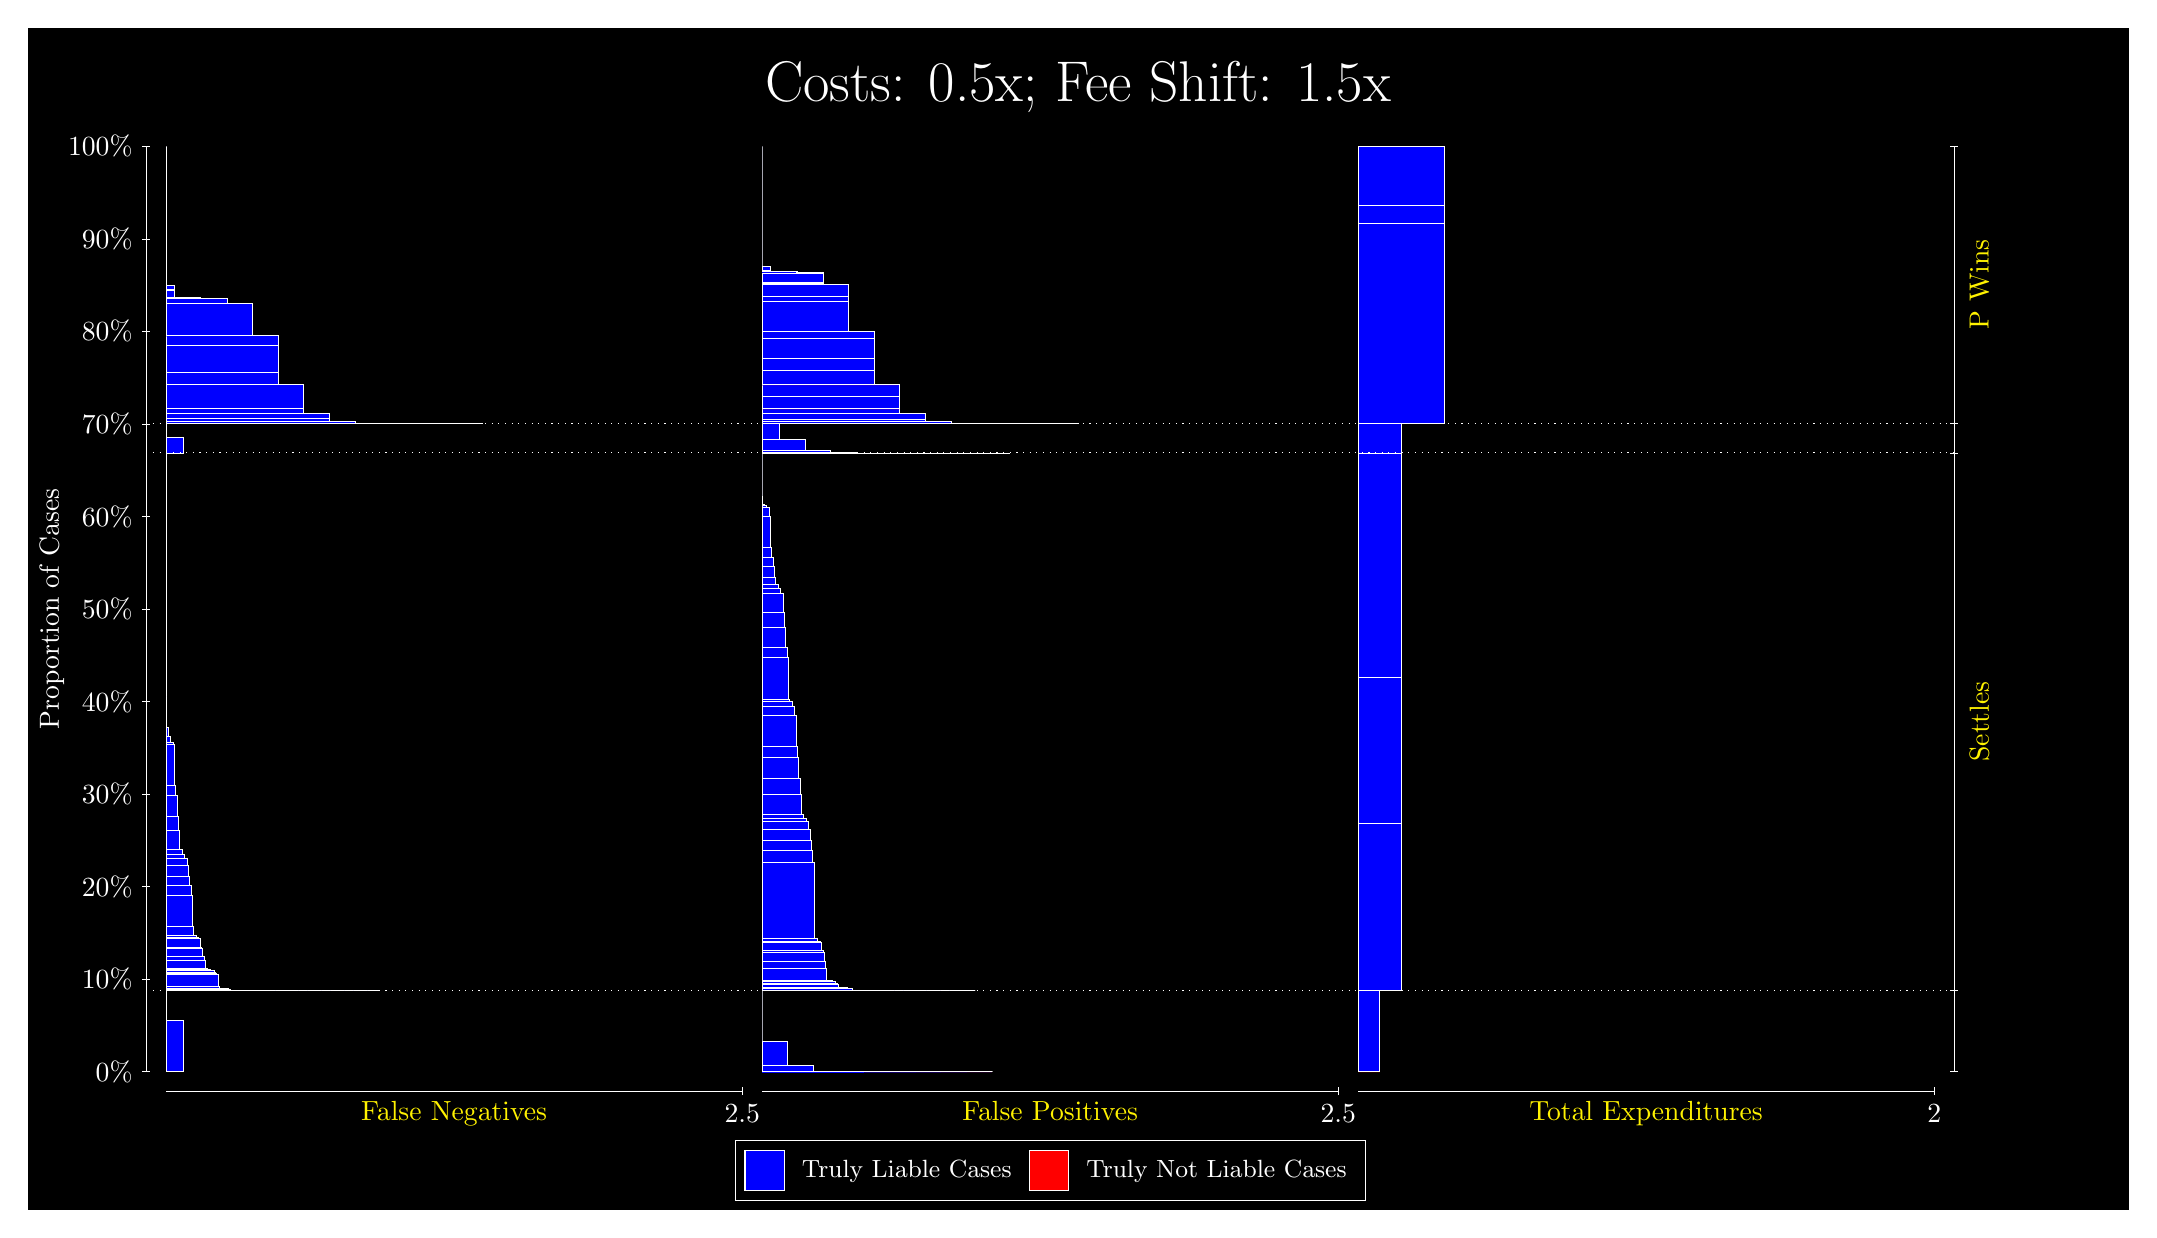
\begin{tikzpicture}
\draw[fill=black] (0,0) rectangle (26.667,15);
\draw[text=white] (0,13.5) rectangle (26.667,15) node[midway] {\huge Costs: 0.5x; Fee Shift: 1.5x};
\draw[white, very thin] (1.5,1.75) -- (1.5,13.5);
\node[rotate=90, text=white, anchor=center] at (0.3, 7.625) {Proportion of Cases};
\draw[white, very thin] (1.45,1.75) -- (1.55,1.75);
\node[text=white, anchor=east] at (1.45, 1.75) {0\%};
\draw[white, very thin] (1.45,2.925) -- (1.55,2.925);
\node[text=white, anchor=east] at (1.45, 2.925) {10\%};
\draw[white, very thin] (1.45,4.1) -- (1.55,4.1);
\node[text=white, anchor=east] at (1.45, 4.1) {20\%};
\draw[white, very thin] (1.45,5.275) -- (1.55,5.275);
\node[text=white, anchor=east] at (1.45, 5.275) {30\%};
\draw[white, very thin] (1.45,6.45) -- (1.55,6.45);
\node[text=white, anchor=east] at (1.45, 6.45) {40\%};
\draw[white, very thin] (1.45,7.625) -- (1.55,7.625);
\node[text=white, anchor=east] at (1.45, 7.625) {50\%};
\draw[white, very thin] (1.45,8.8) -- (1.55,8.8);
\node[text=white, anchor=east] at (1.45, 8.8) {60\%};
\draw[white, very thin] (1.45,9.975) -- (1.55,9.975);
\node[text=white, anchor=east] at (1.45, 9.975) {70\%};
\draw[white, very thin] (1.45,11.15) -- (1.55,11.15);
\node[text=white, anchor=east] at (1.45, 11.15) {80\%};
\draw[white, very thin] (1.45,12.325) -- (1.55,12.325);
\node[text=white, anchor=east] at (1.45, 12.325) {90\%};
\draw[white, very thin] (1.45,13.5) -- (1.55,13.5);
\node[text=white, anchor=east] at (1.45, 13.5) {100\%};

\draw[white, very thin] (24.457,1.75) -- (24.457,13.5);
\draw[white, very thin] (24.407,1.75) -- (24.507,1.75);
\node[anchor=west] at (24.407, 1.75) {};
\draw[white, very thin] (24.407,2.7841) -- (24.507,2.7841);
\node[anchor=west] at (24.407, 2.7841) {};
\draw[white, very thin] (24.407,9.6074) -- (24.507,9.6074);
\node[anchor=west] at (24.407, 9.6074) {};
\draw[white, very thin] (24.407,9.9834) -- (24.507,9.9834);
\node[anchor=west] at (24.407, 9.9834) {};
\draw[white, very thin] (24.407,13.5) -- (24.507,13.5);
\node[anchor=west] at (24.407, 13.5) {};

\draw[white, very thin, fill=blue] (1.75,1.75) rectangle (1.9696,2.4007);
\draw[white, very thin, fill=red] (1.75,2.4007) rectangle (1.75,2.4007);
\draw[white, very thin, fill=blue] (1.75,2.4007) rectangle (1.75,2.7841);
\draw[white, very thin, fill=blue] (1.75,2.7841) rectangle (4.458,2.7841);
\draw[white, very thin, fill=blue] (1.75,2.7841) rectangle (4.3116,2.7841);
\draw[white, very thin, fill=blue] (1.75,2.7841) rectangle (4.1652,2.7841);
\draw[white, very thin, fill=blue] (1.75,2.7841) rectangle (4.1327,2.7841);
\draw[white, very thin, fill=blue] (1.75,2.7841) rectangle (4.0188,2.7841);
\draw[white, very thin, fill=blue] (1.75,2.7841) rectangle (3.9863,2.7841);
\draw[white, very thin, fill=blue] (1.75,2.7841) rectangle (3.8725,2.7841);
\draw[white, very thin, fill=blue] (1.75,2.7841) rectangle (3.8399,2.7841);
\draw[white, very thin, fill=blue] (1.75,2.7841) rectangle (3.8074,2.7841);
\draw[white, very thin, fill=blue] (1.75,2.7841) rectangle (3.7261,2.7841);
\draw[white, very thin, fill=blue] (1.75,2.7841) rectangle (3.6936,2.7841);
\draw[white, very thin, fill=blue] (1.75,2.7841) rectangle (3.661,2.7841);
\draw[white, very thin, fill=blue] (1.75,2.7841) rectangle (3.5797,2.7841);
\draw[white, very thin, fill=blue] (1.75,2.7841) rectangle (3.5472,2.7841);
\draw[white, very thin, fill=blue] (1.75,2.7841) rectangle (3.5147,2.7841);
\draw[white, very thin, fill=blue] (1.75,2.7841) rectangle (3.4821,2.7841);
\draw[white, very thin, fill=blue] (1.75,2.7841) rectangle (3.4333,2.7841);
\draw[white, very thin, fill=blue] (1.75,2.7841) rectangle (3.4008,2.7841);
\draw[white, very thin, fill=blue] (1.75,2.7841) rectangle (3.3683,2.7841);
\draw[white, very thin, fill=blue] (1.75,2.7841) rectangle (3.3358,2.7841);
\draw[white, very thin, fill=blue] (1.75,2.7841) rectangle (3.287,2.7841);
\draw[white, very thin, fill=blue] (1.75,2.7841) rectangle (3.2544,2.7841);
\draw[white, very thin, fill=blue] (1.75,2.7841) rectangle (3.2219,2.7841);
\draw[white, very thin, fill=blue] (1.75,2.7841) rectangle (3.1894,2.7841);
\draw[white, very thin, fill=blue] (1.75,2.7841) rectangle (3.1568,2.7841);
\draw[white, very thin, fill=blue] (1.75,2.7841) rectangle (3.1406,2.7841);
\draw[white, very thin, fill=blue] (1.75,2.7841) rectangle (3.1081,2.7841);
\draw[white, very thin, fill=blue] (1.75,2.7841) rectangle (3.0755,2.7841);
\draw[white, very thin, fill=blue] (1.75,2.7841) rectangle (3.043,2.7841);
\draw[white, very thin, fill=blue] (1.75,2.7841) rectangle (3.0105,2.7841);
\draw[white, very thin, fill=blue] (1.75,2.7841) rectangle (2.9942,2.7841);
\draw[white, very thin, fill=blue] (1.75,2.7841) rectangle (2.9617,2.7841);
\draw[white, very thin, fill=blue] (1.75,2.7841) rectangle (2.9292,2.7841);
\draw[white, very thin, fill=blue] (1.75,2.7841) rectangle (2.8966,2.7841);
\draw[white, very thin, fill=blue] (1.75,2.7841) rectangle (2.8641,2.7842);
\draw[white, very thin, fill=blue] (1.75,2.7842) rectangle (2.8478,2.7842);
\draw[white, very thin, fill=blue] (1.75,2.7842) rectangle (2.8316,2.7843);
\draw[white, very thin, fill=blue] (1.75,2.7843) rectangle (2.8153,2.7843);
\draw[white, very thin, fill=blue] (1.75,2.7843) rectangle (2.7828,2.7843);
\draw[white, very thin, fill=blue] (1.75,2.7843) rectangle (2.7502,2.7847);
\draw[white, very thin, fill=blue] (1.75,2.7847) rectangle (2.7177,2.7852);
\draw[white, very thin, fill=blue] (1.75,2.7852) rectangle (2.7015,2.7855);
\draw[white, very thin, fill=blue] (1.75,2.7855) rectangle (2.6852,2.7859);
\draw[white, very thin, fill=blue] (1.75,2.7859) rectangle (2.6689,2.786);
\draw[white, very thin, fill=blue] (1.75,2.786) rectangle (2.6364,2.7862);
\draw[white, very thin, fill=blue] (1.75,2.7862) rectangle (2.6039,2.7875);
\draw[white, very thin, fill=blue] (1.75,2.7875) rectangle (2.5713,2.7935);
\draw[white, very thin, fill=blue] (1.75,2.7935) rectangle (2.5551,2.798);
\draw[white, very thin, fill=blue] (1.75,2.798) rectangle (2.5388,2.804);
\draw[white, very thin, fill=blue] (1.75,2.804) rectangle (2.5225,2.8045);
\draw[white, very thin, fill=blue] (1.75,2.8045) rectangle (2.5063,2.8097);
\draw[white, very thin, fill=blue] (1.75,2.8097) rectangle (2.49,2.8104);
\draw[white, very thin, fill=blue] (1.75,2.8104) rectangle (2.4575,2.8122);
\draw[white, very thin, fill=blue] (1.75,2.8122) rectangle (2.425,2.8296);
\draw[white, very thin, fill=blue] (1.75,2.8296) rectangle (2.4087,2.9812);
\draw[white, very thin, fill=blue] (1.75,2.9812) rectangle (2.3924,3.001);
\draw[white, very thin, fill=blue] (1.75,3.001) rectangle (2.3762,3.0111);
\draw[white, very thin, fill=blue] (1.75,3.0111) rectangle (2.3599,3.03);
\draw[white, very thin, fill=blue] (1.75,3.03) rectangle (2.3436,3.036);
\draw[white, very thin, fill=blue] (1.75,3.036) rectangle (2.3111,3.0439);
\draw[white, very thin, fill=blue] (1.75,3.0439) rectangle (2.2786,3.0671);
\draw[white, very thin, fill=blue] (1.75,3.0671) rectangle (2.2461,3.1624);
\draw[white, very thin, fill=blue] (1.75,3.1624) rectangle (2.2298,3.2135);
\draw[white, very thin, fill=blue] (1.75,3.2135) rectangle (2.2135,3.3118);
\draw[white, very thin, fill=blue] (1.75,3.3118) rectangle (2.1973,3.3304);
\draw[white, very thin, fill=blue] (1.75,3.3304) rectangle (2.181,3.4391);
\draw[white, very thin, fill=blue] (1.75,3.4391) rectangle (2.1647,3.4494);
\draw[white, very thin, fill=blue] (1.75,3.4494) rectangle (2.1322,3.4783);
\draw[white, very thin, fill=blue] (1.75,3.4783) rectangle (2.0997,3.5897);
\draw[white, very thin, fill=blue] (1.75,3.5897) rectangle (2.0834,3.985);
\draw[white, very thin, fill=blue] (1.75,3.985) rectangle (2.0672,4.1117);
\draw[white, very thin, fill=blue] (1.75,4.1117) rectangle (2.0509,4.2294);
\draw[white, very thin, fill=blue] (1.75,4.2294) rectangle (2.0346,4.3672);
\draw[white, very thin, fill=blue] (1.75,4.3672) rectangle (2.0184,4.4543);
\draw[white, very thin, fill=blue] (1.75,4.4543) rectangle (1.9858,4.5043);
\draw[white, very thin, fill=blue] (1.75,4.5043) rectangle (1.9533,4.5735);
\draw[white, very thin, fill=blue] (1.75,4.5735) rectangle (1.9208,4.8138);
\draw[white, very thin, fill=blue] (1.75,4.8138) rectangle (1.9045,4.9934);
\draw[white, very thin, fill=blue] (1.75,4.9934) rectangle (1.8882,5.2537);
\draw[white, very thin, fill=blue] (1.75,5.2537) rectangle (1.872,5.3817);
\draw[white, very thin, fill=blue] (1.75,5.3817) rectangle (1.8557,5.9082);
\draw[white, very thin, fill=blue] (1.75,5.9082) rectangle (1.8395,5.9333);
\draw[white, very thin, fill=blue] (1.75,5.9333) rectangle (1.8069,6.0063);
\draw[white, very thin, fill=blue] (1.75,6.0063) rectangle (1.7744,6.122);
\draw[white, very thin, fill=blue] (1.75,6.122) rectangle (1.7581,6.5132);
\draw[white, very thin, fill=red] (1.75,6.5132) rectangle (1.75,6.5132);
\draw[white, very thin, fill=blue] (1.75,6.5132) rectangle (1.75,9.6074);
\draw[white, very thin, fill=blue] (1.75,9.6074) rectangle (1.9696,9.8068);
\draw[white, very thin, fill=red] (1.75,9.8068) rectangle (1.75,9.8068);
\draw[white, very thin, fill=blue] (1.75,9.8068) rectangle (1.75,9.9834);
\draw[white, very thin, fill=blue] (1.75,9.9834) rectangle (5.7754,9.9834);
\draw[white, very thin, fill=blue] (1.75,9.9834) rectangle (5.4501,9.9834);
\draw[white, very thin, fill=blue] (1.75,9.9834) rectangle (5.1248,9.9834);
\draw[white, very thin, fill=blue] (1.75,9.9834) rectangle (4.7995,9.9835);
\draw[white, very thin, fill=blue] (1.75,9.9835) rectangle (4.7995,9.9836);
\draw[white, very thin, fill=blue] (1.75,9.9836) rectangle (4.4742,9.9859);
\draw[white, very thin, fill=blue] (1.75,9.9859) rectangle (4.149,10.006);
\draw[white, very thin, fill=blue] (1.75,10.006) rectangle (3.8237,10.049);
\draw[white, very thin, fill=blue] (1.75,10.049) rectangle (3.8237,10.116);
\draw[white, very thin, fill=blue] (1.75,10.116) rectangle (3.8074,10.116);
\draw[white, very thin, fill=blue] (1.75,10.116) rectangle (3.4984,10.168);
\draw[white, very thin, fill=blue] (1.75,10.168) rectangle (3.4984,10.479);
\draw[white, very thin, fill=blue] (1.75,10.479) rectangle (3.4821,10.479);
\draw[white, very thin, fill=blue] (1.75,10.479) rectangle (3.1731,10.627);
\draw[white, very thin, fill=blue] (1.75,10.627) rectangle (3.1731,10.975);
\draw[white, very thin, fill=blue] (1.75,10.975) rectangle (3.1731,11.097);
\draw[white, very thin, fill=blue] (1.75,11.097) rectangle (3.1568,11.097);
\draw[white, very thin, fill=blue] (1.75,11.097) rectangle (3.1568,11.097);
\draw[white, very thin, fill=blue] (1.75,11.097) rectangle (2.8478,11.504);
\draw[white, very thin, fill=blue] (1.75,11.504) rectangle (2.8316,11.504);
\draw[white, very thin, fill=blue] (1.75,11.504) rectangle (2.5225,11.508);
\draw[white, very thin, fill=blue] (1.75,11.508) rectangle (2.5225,11.568);
\draw[white, very thin, fill=blue] (1.75,11.568) rectangle (2.5225,11.574);
\draw[white, very thin, fill=blue] (1.75,11.574) rectangle (2.5063,11.574);
\draw[white, very thin, fill=blue] (1.75,11.574) rectangle (2.5063,11.574);
\draw[white, very thin, fill=blue] (1.75,11.574) rectangle (2.1973,11.575);
\draw[white, very thin, fill=blue] (1.75,11.575) rectangle (2.1973,11.575);
\draw[white, very thin, fill=blue] (1.75,11.575) rectangle (2.181,11.581);
\draw[white, very thin, fill=blue] (1.75,11.581) rectangle (1.872,11.581);
\draw[white, very thin, fill=blue] (1.75,11.581) rectangle (1.872,11.581);
\draw[white, very thin, fill=blue] (1.75,11.581) rectangle (1.8557,11.669);
\draw[white, very thin, fill=blue] (1.75,11.669) rectangle (1.8557,11.685);
\draw[white, very thin, fill=blue] (1.75,11.685) rectangle (1.8557,11.736);
\draw[white, very thin, fill=red] (1.75,11.736) rectangle (1.75,11.736);
\draw[white, very thin, fill=blue] (1.75,11.736) rectangle (1.75,13.5);
\draw[white, very thin, fill=red] (9.3189,1.75) rectangle (12.246,1.75);
\draw[white, very thin, fill=blue] (9.3189,1.75) rectangle (12.246,1.75);
\draw[white, very thin, fill=blue] (9.3189,1.75) rectangle (11.921,1.75);
\draw[white, very thin, fill=blue] (9.3189,1.75) rectangle (11.596,1.75);
\draw[white, very thin, fill=blue] (9.3189,1.75) rectangle (11.271,1.75);
\draw[white, very thin, fill=blue] (9.3189,1.75) rectangle (10.945,1.75);
\draw[white, very thin, fill=blue] (9.3189,1.75) rectangle (10.62,1.7503);
\draw[white, very thin, fill=blue] (9.3189,1.7503) rectangle (10.295,1.7573);
\draw[white, very thin, fill=blue] (9.3189,1.7573) rectangle (9.9694,1.829);
\draw[white, very thin, fill=blue] (9.3189,1.829) rectangle (9.6442,2.1333);
\draw[white, very thin, fill=blue] (9.3189,2.1333) rectangle (9.3189,2.7841);
\draw[white, very thin, fill=red] (9.3189,2.7841) rectangle (12.027,2.7841);
\draw[white, very thin, fill=blue] (9.3189,2.7841) rectangle (12.027,2.7841);
\draw[white, very thin, fill=red] (9.3189,2.7841) rectangle (11.88,2.7841);
\draw[white, very thin, fill=blue] (9.3189,2.7841) rectangle (11.88,2.7841);
\draw[white, very thin, fill=red] (9.3189,2.7841) rectangle (11.734,2.7841);
\draw[white, very thin, fill=blue] (9.3189,2.7841) rectangle (11.734,2.7841);
\draw[white, very thin, fill=blue] (9.3189,2.7841) rectangle (11.702,2.7841);
\draw[white, very thin, fill=red] (9.3189,2.7841) rectangle (11.588,2.7841);
\draw[white, very thin, fill=blue] (9.3189,2.7841) rectangle (11.588,2.7841);
\draw[white, very thin, fill=blue] (9.3189,2.7841) rectangle (11.555,2.7841);
\draw[white, very thin, fill=red] (9.3189,2.7841) rectangle (11.441,2.7841);
\draw[white, very thin, fill=blue] (9.3189,2.7841) rectangle (11.441,2.7841);
\draw[white, very thin, fill=blue] (9.3189,2.7841) rectangle (11.409,2.7841);
\draw[white, very thin, fill=blue] (9.3189,2.7841) rectangle (11.376,2.7841);
\draw[white, very thin, fill=red] (9.3189,2.7841) rectangle (11.295,2.7841);
\draw[white, very thin, fill=blue] (9.3189,2.7841) rectangle (11.295,2.7841);
\draw[white, very thin, fill=blue] (9.3189,2.7841) rectangle (11.262,2.7841);
\draw[white, very thin, fill=blue] (9.3189,2.7841) rectangle (11.23,2.7841);
\draw[white, very thin, fill=red] (9.3189,2.7841) rectangle (11.149,2.7841);
\draw[white, very thin, fill=blue] (9.3189,2.7841) rectangle (11.149,2.7841);
\draw[white, very thin, fill=blue] (9.3189,2.7841) rectangle (11.116,2.7841);
\draw[white, very thin, fill=blue] (9.3189,2.7841) rectangle (11.084,2.7841);
\draw[white, very thin, fill=blue] (9.3189,2.7841) rectangle (11.051,2.7841);
\draw[white, very thin, fill=red] (9.3189,2.7841) rectangle (11.002,2.7841);
\draw[white, very thin, fill=blue] (9.3189,2.7841) rectangle (11.002,2.7841);
\draw[white, very thin, fill=blue] (9.3189,2.7841) rectangle (10.97,2.7841);
\draw[white, very thin, fill=blue] (9.3189,2.7841) rectangle (10.937,2.7841);
\draw[white, very thin, fill=blue] (9.3189,2.7841) rectangle (10.905,2.7841);
\draw[white, very thin, fill=red] (9.3189,2.7841) rectangle (10.856,2.7841);
\draw[white, very thin, fill=blue] (9.3189,2.7841) rectangle (10.856,2.7841);
\draw[white, very thin, fill=blue] (9.3189,2.7841) rectangle (10.823,2.7841);
\draw[white, very thin, fill=blue] (9.3189,2.7841) rectangle (10.791,2.7844);
\draw[white, very thin, fill=blue] (9.3189,2.7844) rectangle (10.758,2.7845);
\draw[white, very thin, fill=blue] (9.3189,2.7845) rectangle (10.726,2.7846);
\draw[white, very thin, fill=red] (9.3189,2.7846) rectangle (10.709,2.7846);
\draw[white, very thin, fill=blue] (9.3189,2.7846) rectangle (10.709,2.7846);
\draw[white, very thin, fill=blue] (9.3189,2.7846) rectangle (10.677,2.7846);
\draw[white, very thin, fill=blue] (9.3189,2.7846) rectangle (10.644,2.7846);
\draw[white, very thin, fill=blue] (9.3189,2.7846) rectangle (10.612,2.7862);
\draw[white, very thin, fill=blue] (9.3189,2.7862) rectangle (10.579,2.7867);
\draw[white, very thin, fill=red] (9.3189,2.7867) rectangle (10.563,2.7867);
\draw[white, very thin, fill=blue] (9.3189,2.7867) rectangle (10.563,2.7868);
\draw[white, very thin, fill=blue] (9.3189,2.7868) rectangle (10.531,2.7869);
\draw[white, very thin, fill=blue] (9.3189,2.7869) rectangle (10.498,2.7871);
\draw[white, very thin, fill=blue] (9.3189,2.7871) rectangle (10.465,2.8035);
\draw[white, very thin, fill=blue] (9.3189,2.8035) rectangle (10.433,2.8116);
\draw[white, very thin, fill=red] (9.3189,2.8116) rectangle (10.417,2.8116);
\draw[white, very thin, fill=blue] (9.3189,2.8116) rectangle (10.417,2.8129);
\draw[white, very thin, fill=blue] (9.3189,2.8129) rectangle (10.4,2.818);
\draw[white, very thin, fill=blue] (9.3189,2.818) rectangle (10.384,2.8187);
\draw[white, very thin, fill=blue] (9.3189,2.8187) rectangle (10.352,2.8205);
\draw[white, very thin, fill=blue] (9.3189,2.8205) rectangle (10.319,2.8211);
\draw[white, very thin, fill=blue] (9.3189,2.8211) rectangle (10.287,2.8575);
\draw[white, very thin, fill=red] (9.3189,2.8575) rectangle (10.27,2.8575);
\draw[white, very thin, fill=blue] (9.3189,2.8575) rectangle (10.27,2.8756);
\draw[white, very thin, fill=blue] (9.3189,2.8756) rectangle (10.254,2.8945);
\draw[white, very thin, fill=blue] (9.3189,2.8945) rectangle (10.238,2.9016);
\draw[white, very thin, fill=blue] (9.3189,2.9016) rectangle (10.205,2.9058);
\draw[white, very thin, fill=blue] (9.3189,2.9058) rectangle (10.173,2.9136);
\draw[white, very thin, fill=blue] (9.3189,2.9136) rectangle (10.14,3.0596);
\draw[white, very thin, fill=red] (9.3189,3.0596) rectangle (10.124,3.0596);
\draw[white, very thin, fill=blue] (9.3189,3.0596) rectangle (10.124,3.1526);
\draw[white, very thin, fill=blue] (9.3189,3.1526) rectangle (10.108,3.2645);
\draw[white, very thin, fill=blue] (9.3189,3.2645) rectangle (10.091,3.2897);
\draw[white, very thin, fill=blue] (9.3189,3.2897) rectangle (10.075,3.3884);
\draw[white, very thin, fill=blue] (9.3189,3.3884) rectangle (10.059,3.4089);
\draw[white, very thin, fill=blue] (9.3189,3.4089) rectangle (10.026,3.4378);
\draw[white, very thin, fill=blue] (9.3189,3.4378) rectangle (9.9938,3.4477);
\draw[white, very thin, fill=red] (9.3189,3.4477) rectangle (9.9776,3.4477);
\draw[white, very thin, fill=blue] (9.3189,3.4477) rectangle (9.9776,4.4066);
\draw[white, very thin, fill=blue] (9.3189,4.4066) rectangle (9.9613,4.5637);
\draw[white, very thin, fill=blue] (9.3189,4.5637) rectangle (9.945,4.6929);
\draw[white, very thin, fill=blue] (9.3189,4.6929) rectangle (9.9288,4.829);
\draw[white, very thin, fill=blue] (9.3189,4.829) rectangle (9.9125,4.9267);
\draw[white, very thin, fill=blue] (9.3189,4.9267) rectangle (9.88,4.9651);
\draw[white, very thin, fill=blue] (9.3189,4.9651) rectangle (9.8475,5.0151);
\draw[white, very thin, fill=blue] (9.3189,5.0151) rectangle (9.8149,5.2694);
\draw[white, very thin, fill=blue] (9.3189,5.2694) rectangle (9.7987,5.4732);
\draw[white, very thin, fill=blue] (9.3189,5.4732) rectangle (9.7824,5.7466);
\draw[white, very thin, fill=blue] (9.3189,5.7466) rectangle (9.7661,5.8782);
\draw[white, very thin, fill=blue] (9.3189,5.8782) rectangle (9.7499,6.2694);
\draw[white, very thin, fill=blue] (9.3189,6.2694) rectangle (9.7336,6.3851);
\draw[white, very thin, fill=blue] (9.3189,6.3851) rectangle (9.7011,6.4581);
\draw[white, very thin, fill=blue] (9.3189,6.4581) rectangle (9.6685,6.4832);
\draw[white, very thin, fill=blue] (9.3189,6.4832) rectangle (9.6523,7.0097);
\draw[white, very thin, fill=blue] (9.3189,7.0097) rectangle (9.636,7.1377);
\draw[white, very thin, fill=blue] (9.3189,7.1377) rectangle (9.6198,7.398);
\draw[white, very thin, fill=blue] (9.3189,7.398) rectangle (9.6035,7.5777);
\draw[white, very thin, fill=blue] (9.3189,7.5777) rectangle (9.5872,7.818);
\draw[white, very thin, fill=blue] (9.3189,7.818) rectangle (9.5547,7.8872);
\draw[white, very thin, fill=blue] (9.3189,7.8872) rectangle (9.5222,7.9371);
\draw[white, very thin, fill=blue] (9.3189,7.9371) rectangle (9.4896,8.0243);
\draw[white, very thin, fill=blue] (9.3189,8.0243) rectangle (9.4734,8.162);
\draw[white, very thin, fill=blue] (9.3189,8.162) rectangle (9.4571,8.2797);
\draw[white, very thin, fill=blue] (9.3189,8.2797) rectangle (9.4408,8.4065);
\draw[white, very thin, fill=blue] (9.3189,8.4065) rectangle (9.4246,8.8017);
\draw[white, very thin, fill=blue] (9.3189,8.8017) rectangle (9.4083,8.9131);
\draw[white, very thin, fill=blue] (9.3189,8.9131) rectangle (9.3758,8.9421);
\draw[white, very thin, fill=blue] (9.3189,8.9421) rectangle (9.3433,8.9523);
\draw[white, very thin, fill=blue] (9.3189,8.9523) rectangle (9.327,9.0611);
\draw[white, very thin, fill=blue] (9.3189,9.0611) rectangle (9.3189,9.6074);
\draw[white, very thin, fill=red] (9.3189,9.6074) rectangle (12.466,9.6074);
\draw[white, very thin, fill=blue] (9.3189,9.6074) rectangle (12.466,9.6074);
\draw[white, very thin, fill=blue] (9.3189,9.6074) rectangle (12.141,9.6074);
\draw[white, very thin, fill=blue] (9.3189,9.6074) rectangle (11.815,9.6074);
\draw[white, very thin, fill=blue] (9.3189,9.6074) rectangle (11.49,9.6074);
\draw[white, very thin, fill=blue] (9.3189,9.6074) rectangle (11.165,9.6074);
\draw[white, very thin, fill=blue] (9.3189,9.6074) rectangle (10.84,9.6074);
\draw[white, very thin, fill=blue] (9.3189,9.6074) rectangle (10.514,9.6089);
\draw[white, very thin, fill=blue] (9.3189,9.6089) rectangle (10.189,9.6408);
\draw[white, very thin, fill=blue] (9.3189,9.6408) rectangle (9.8637,9.784);
\draw[white, very thin, fill=blue] (9.3189,9.784) rectangle (9.5384,9.9834);
\draw[white, very thin, fill=red] (9.3189,9.9834) rectangle (13.344,9.9834);
\draw[white, very thin, fill=blue] (9.3189,9.9834) rectangle (13.344,9.9834);
\draw[white, very thin, fill=red] (9.3189,9.9834) rectangle (13.019,9.9834);
\draw[white, very thin, fill=blue] (9.3189,9.9834) rectangle (13.019,9.9834);
\draw[white, very thin, fill=red] (9.3189,9.9834) rectangle (12.694,9.9834);
\draw[white, very thin, fill=blue] (9.3189,9.9834) rectangle (12.694,9.9834);
\draw[white, very thin, fill=blue] (9.3189,9.9834) rectangle (12.368,9.9835);
\draw[white, very thin, fill=red] (9.3189,9.9835) rectangle (12.368,9.9835);
\draw[white, very thin, fill=blue] (9.3189,9.9835) rectangle (12.368,9.9836);
\draw[white, very thin, fill=red] (9.3189,9.9836) rectangle (12.043,9.9836);
\draw[white, very thin, fill=blue] (9.3189,9.9836) rectangle (12.043,9.9851);
\draw[white, very thin, fill=blue] (9.3189,9.9851) rectangle (12.043,9.9856);
\draw[white, very thin, fill=blue] (9.3189,9.9856) rectangle (12.043,9.986);
\draw[white, very thin, fill=red] (9.3189,9.986) rectangle (11.718,9.986);
\draw[white, very thin, fill=blue] (9.3189,9.986) rectangle (11.718,10.003);
\draw[white, very thin, fill=blue] (9.3189,10.003) rectangle (11.718,10.007);
\draw[white, very thin, fill=blue] (9.3189,10.007) rectangle (11.393,10.039);
\draw[white, very thin, fill=red] (9.3189,10.039) rectangle (11.393,10.039);
\draw[white, very thin, fill=blue] (9.3189,10.039) rectangle (11.393,10.115);
\draw[white, very thin, fill=red] (9.3189,10.115) rectangle (11.376,10.115);
\draw[white, very thin, fill=blue] (9.3189,10.115) rectangle (11.376,10.115);
\draw[white, very thin, fill=blue] (9.3189,10.115) rectangle (11.067,10.169);
\draw[white, very thin, fill=red] (9.3189,10.169) rectangle (11.067,10.169);
\draw[white, very thin, fill=blue] (9.3189,10.169) rectangle (11.067,10.323);
\draw[white, very thin, fill=blue] (9.3189,10.323) rectangle (11.067,10.474);
\draw[white, very thin, fill=blue] (9.3189,10.474) rectangle (11.051,10.474);
\draw[white, very thin, fill=red] (9.3189,10.474) rectangle (11.051,10.474);
\draw[white, very thin, fill=blue] (9.3189,10.474) rectangle (11.051,10.474);
\draw[white, very thin, fill=blue] (9.3189,10.474) rectangle (10.742,10.653);
\draw[white, very thin, fill=blue] (9.3189,10.653) rectangle (10.742,10.805);
\draw[white, very thin, fill=blue] (9.3189,10.805) rectangle (10.742,11.058);
\draw[white, very thin, fill=blue] (9.3189,11.058) rectangle (10.742,11.155);
\draw[white, very thin, fill=red] (9.3189,11.155) rectangle (10.726,11.155);
\draw[white, very thin, fill=blue] (9.3189,11.155) rectangle (10.726,11.155);
\draw[white, very thin, fill=blue] (9.3189,11.155) rectangle (10.726,11.155);
\draw[white, very thin, fill=blue] (9.3189,11.155) rectangle (10.417,11.53);
\draw[white, very thin, fill=blue] (9.3189,11.53) rectangle (10.417,11.601);
\draw[white, very thin, fill=blue] (9.3189,11.601) rectangle (10.417,11.747);
\draw[white, very thin, fill=blue] (9.3189,11.747) rectangle (10.4,11.747);
\draw[white, very thin, fill=red] (9.3189,11.747) rectangle (10.4,11.747);
\draw[white, very thin, fill=blue] (9.3189,11.747) rectangle (10.4,11.747);
\draw[white, very thin, fill=blue] (9.3189,11.747) rectangle (10.091,11.764);
\draw[white, very thin, fill=blue] (9.3189,11.764) rectangle (10.091,11.779);
\draw[white, very thin, fill=blue] (9.3189,11.779) rectangle (10.091,11.886);
\draw[white, very thin, fill=blue] (9.3189,11.886) rectangle (10.091,11.903);
\draw[white, very thin, fill=blue] (9.3189,11.903) rectangle (10.075,11.903);
\draw[white, very thin, fill=blue] (9.3189,11.903) rectangle (10.075,11.903);
\draw[white, very thin, fill=red] (9.3189,11.903) rectangle (10.075,11.903);
\draw[white, very thin, fill=blue] (9.3189,11.903) rectangle (10.075,11.903);
\draw[white, very thin, fill=blue] (9.3189,11.903) rectangle (9.7661,11.905);
\draw[white, very thin, fill=blue] (9.3189,11.905) rectangle (9.7661,11.909);
\draw[white, very thin, fill=blue] (9.3189,11.909) rectangle (9.7499,11.909);
\draw[white, very thin, fill=blue] (9.3189,11.909) rectangle (9.7499,11.909);
\draw[white, very thin, fill=red] (9.3189,11.909) rectangle (9.7499,11.909);
\draw[white, very thin, fill=blue] (9.3189,11.909) rectangle (9.7499,11.909);
\draw[white, very thin, fill=blue] (9.3189,11.909) rectangle (9.7499,11.91);
\draw[white, very thin, fill=blue] (9.3189,11.91) rectangle (9.4408,11.91);
\draw[white, very thin, fill=blue] (9.3189,11.91) rectangle (9.4408,11.91);
\draw[white, very thin, fill=blue] (9.3189,11.91) rectangle (9.4408,11.91);
\draw[white, very thin, fill=blue] (9.3189,11.91) rectangle (9.4246,11.916);
\draw[white, very thin, fill=blue] (9.3189,11.916) rectangle (9.4246,11.93);
\draw[white, very thin, fill=red] (9.3189,11.93) rectangle (9.4246,11.93);
\draw[white, very thin, fill=blue] (9.3189,11.93) rectangle (9.4246,11.971);
\draw[white, very thin, fill=blue] (9.3189,11.971) rectangle (9.4246,11.98);
\draw[white, very thin, fill=red] (9.3189,11.98) rectangle (9.3189,11.98);
\draw[white, very thin, fill=blue] (9.3189,11.98) rectangle (9.3189,13.5);
\draw[white, very thin, fill=red] (16.888,1.75) rectangle (17.162,1.75);
\draw[white, very thin, fill=blue] (16.888,1.75) rectangle (17.162,2.7841);
\draw[white, very thin, fill=red] (16.888,2.7841) rectangle (17.437,2.7841);
\draw[white, very thin, fill=blue] (16.888,2.7841) rectangle (17.437,4.9042);
\draw[white, very thin, fill=red] (16.888,4.9042) rectangle (17.437,4.9042);
\draw[white, very thin, fill=blue] (16.888,4.9042) rectangle (17.437,6.7543);
\draw[white, very thin, fill=red] (16.888,6.7543) rectangle (17.437,6.7543);
\draw[white, very thin, fill=blue] (16.888,6.7543) rectangle (17.437,9.6074);
\draw[white, very thin, fill=red] (16.888,9.6074) rectangle (17.437,9.6074);
\draw[white, very thin, fill=blue] (16.888,9.6074) rectangle (17.437,9.9834);
\draw[white, very thin, fill=red] (16.888,9.9834) rectangle (17.986,9.9834);
\draw[white, very thin, fill=blue] (16.888,9.9834) rectangle (17.986,12.52);
\draw[white, very thin, fill=red] (16.888,12.52) rectangle (17.986,12.52);
\draw[white, very thin, fill=blue] (16.888,12.52) rectangle (17.986,12.752);
\draw[white, very thin, fill=red] (16.888,12.752) rectangle (17.986,12.752);
\draw[white, very thin, fill=blue] (16.888,12.752) rectangle (17.986,13.5);
\draw[white, dotted] (1.5,2.7841) -- (24.457,2.7841);
\draw[white, dotted] (1.5,9.6074) -- (24.457,9.6074);
\draw[white, dotted] (1.5,9.9834) -- (24.457,9.9834);
\draw[white, very thin] (1.75,1.5) -- (9.0689,1.5);
\node[text=yellow, anchor=north] at (5.4094, 1.5) {False Negatives};
\draw[white, very thin] (9.0689,1.45) -- (9.0689,1.55);
\node[text=white, anchor=north] at (9.0689, 1.45) {2.5};

\draw[white, very thin] (9.3189,1.5) -- (16.638,1.5);
\node[text=yellow, anchor=north] at (12.978, 1.5) {False Positives};
\draw[white, very thin] (16.638,1.45) -- (16.638,1.55);
\node[text=white, anchor=north] at (16.638, 1.45) {2.5};

\draw[white, very thin] (16.888,1.5) -- (24.207,1.5);
\node[text=yellow, anchor=north] at (20.547, 1.5) {Total Expenditures};
\draw[white, very thin] (24.207,1.45) -- (24.207,1.55);
\node[text=white, anchor=north] at (24.207, 1.45) {2};


\node[text=yellow, centered, rotate=90] at (24.777, 6.1957) {Settles};

\node[text=yellow, centered, rotate=90] at (24.777, 11.742) {P Wins};

\draw (12.978300999999998,1.5) node[draw=none] (baseCoordinate) {};
\begin{scope}[align=center]
        \matrix[scale=0.5, draw=white, below=0.5cm of baseCoordinate, nodes={draw}, column sep=0.1cm]{
            \node[rectangle, draw, minimum width=0.5cm, minimum height=0.5cm, fill=blue] {}; &
            \node[draw=none, font=\small, text=white] (B) {Truly Liable Cases}; &
            \node[rectangle, draw, minimum width=0.5cm, minimum height=0.5cm, fill=red] {}; &
            \node[draw=none, font=\small, text=white] (B) {Truly Not Liable Cases}; \\
            };
\end{scope}

\end{tikzpicture}
\end{document}